%% LyX 2.1.4 created this file.  For more info, see http://www.lyx.org/.
%% Do not edit unless you really know what you are doing.
\documentclass[conference]{IEEEtran}
\usepackage[latin9]{inputenc}
\pagestyle{headings}
\usepackage{amsmath}
\usepackage{graphicx}

\makeatletter
%%%%%%%%%%%%%%%%%%%%%%%%%%%%%% User specified LaTeX commands.


\hyphenation{op-tical net-works semi-conduc-tor}

\newcommand{\MYfooter}{\smash{
\hfil\parbox[t][\height][t]{\textwidth}{}\hfil\hbox{}}}

\def\ps@IEEEtitlepagestyle{%
\def\@oddhead{\mbox{}2016 ICSEE International Conference on the Science of Electrical Engineering \rightmark \hfil }%
\def\@oddfoot{\MYfooter}%
\def\@evenfoot{\MYfooter}}


% adjust as needed
\addtolength{\footskip}{0\baselineskip}
\addtolength{\textheight}{-1\baselineskip}

\makeatother

\begin{document}

\title{A warning about the use of reduced models of synchronous generators }


\author{\IEEEauthorblockN{Elad Venezian} \IEEEauthorblockA{School of EE, Tel Aviv University\\
Ramat Aviv 69978, Israel} \and \IEEEauthorblockN{George Weiss} \IEEEauthorblockA{School of EE, Tel Aviv University\\
Ramat Aviv 69978, Israel} }

\maketitle
%\boldmath
\begin{abstract}
Synchronous generators are an essential component of the electric
grid. Recently, the stability of the electric grid has become an area
of high interest and intensive research. One reason is that the power
grid which has traditionally relied on synchronous generators as its
power source, is changing and becoming more and more based on other
sources. mostly because of the usage of renewable energy sources.

In this work we discuss the stability of a single generator connected
to an infinite bus, and show that reduced models fail to predict the
behavior of this system.
\end{abstract}


\section{Introduction}

% no \IEEEPARstart 

The AC electricity grid was developed at the end of the XIX century,
and basically remained very similar till our days. Many techniques
and models that have been developed in order to analyze and design
the grid and its components are based on assumptions and methods,
which were driven by experience and observations \cite{SauerPai1998}.
In recent years, there is a trend of increasing use of renewable energy,
which requires the conversion of the energy in order to interface
with the power grid. When the rate of the converted energy will become
a significant part, it is not clear whether the traditional models
and methods for controlling the power grid will succeed to control
it \cite{ZhongWeiss2011,DePersiVanDerSchaft2016}. Therefore, there
is an increasing interest in the fundamental mathematical models of
the electrical grid.

\textit{Synchronous generator} (SG) is the main power source of the
electricity grid. The mathematical model of a SG is very complex and
difficult to use. This makes the electric grid to such a complicated
nonlinear and time-varying system that any attempt to prove its stability
analytically is hopeless. Stability analysis is usually done either
by simulation, or analytically on simplified models, in which the
SGs are connected in a simple network and each SG is represented by
reduced order equations, see for instance \cite{DorflerBullo2012}
and \cite{PorcoDorfleBullo2013}. The reduced model of a SG is often
obtained by treating the stator currents as fast variables, thus eliminating
them from the state variables via the singular perturbation approach
(see, for instance, \cite{Khalil}) and keeping only the rotor angle,
and the rotor angular velocity as relevant state variables, see for
instance \cite{Kundur} and \cite{SauerPai1998}.

SGs has the important property that once they synchronize, that is
their rotors spin in the same velocity, they tend to remain synchronized
even without any control. This is important attribute because the
electricity grid must maintain constant frequency, and because the
ability of a SG to transfer constant power through the grid exists
only when the phase difference between each SG and the grid is constant.
Therefore, it is desirable to know if for a given grid which contains
SGs and a loads,all the SGs and tend to synchronize and if the grid
frequency remains constant. In order to use the control stability
analysis, and because the trajectory of the state of a SG in the steady
state is sinusoidal, it is common to use transformation of the voltages
and currents that map sinusoidal trajectory into a constant point
on the state plane. The famous Park's transformation meets this requirement,
so after applying Park's transformation on the SG model, system that
oscillate with fixed sinusoidal oscillation will translated to stable
system. The question whether the system is stable (which means that
all the SGs are synchronized and remain at constant frequency) is
known as frequency stability.

The most common model, which known as the classical model, is a second
order non linear model. \cite{DePersiVanDerSchaft2016} showed that
this model is not realistic enough and that more complicated model,
which known as the \emph{improved swing equation }model should be
used. In this paper we show that even this model is not enough, because
it can't predict a behavior that is predicted by more complicated
model.

The rest of this paper is organized as follows. In Section II, a fourth
order model of SG connected to infinite bus is presented. The reduction
from the fourth order model to the second order \emph{improved swing
equation }is described in Section III. Simulations and local stability
analysis that shows different behavior of the models are given in
Section IV. In Section V we conclude and discuss future directions.% You must have at least 2 lines in the paragraph with the drop letter% (should never be an issue)

\hfill{}

\hfill{}


\section{Modeling SG connected to infinite bus}

In this section we derive the equations for a SG connected to infinite
bus. We start with deriving the equations for single SG, assuming
constant field current. Then, we derive the equations for a single
SG connected to an infinite bus. 


\subsection{Single SG dynamics}

Mathematical models for synchronous machines can be found for instance
in \cite{Kundur},\cite{CaliskanTabuada2014},\cite{SauerPai1998}
and \cite{ZhongWeiss2011}. At this section, we follow the derivations
of \cite{ZhongWeiss2011}. 

Synchronous generator consist of two parts: rotor and stator. The
rotor is a rotated winding that spins inside the stator with an angle
$\theta$ with respect to its initial angle. The rotor can be considered
as a coil with self inductance $L_{f}$ and resistance $R_{f}$ and
a voltage $V_{f}$ across its terminals. The stator consists of three
identical windings that are connected in a star. We consider a generator
without neutral connection and no damper windings. The stator windings
can be regarded as connected coils with self inductance $L$, mutual
inductance $-M$, and resistance $R_{s}$. The negative sign of $-M$
is due to the $2\pi/3$ phase angle between the phases as shown in
Figure \ref{fig:structOfSG}. The amplitude of the mutual inductance
between the rotor and each of the stators windings is $M_{f}$ (which
is a function of $\theta$). We assume no magnetic saturation effects
in the iron core and no Eddy currents. The stator terminals are labeled
with the letters a,b,c and the voltages across the stator terminals
are denoted by $v=\left[\begin{array}{c}
v_{a}\\
v_{b}\\
v_{c}
\end{array}\right]$. 

Lets define the vectors $\widetilde{\cos}\theta=\left[\begin{array}{c}
\cos\left(\theta\right)\\
\cos\left(\theta-\frac{2\pi}{3}\right)\\
\cos\left(\theta-\frac{4\pi}{3}\right)
\end{array}\right]$ and $\widetilde{\sin}\theta=\left[\begin{array}{c}
\sin\left(\theta\right)\\
\sin\left(\theta-\frac{2\pi}{3}\right)\\
\sin\left(\theta-\frac{4\pi}{3}\right)
\end{array}\right]$. We denote the stator flux by $\Phi=\left[\begin{array}{c}
\Phi_{a}\\
\Phi_{b}\\
\Phi_{c}
\end{array}\right]$, the stator currents by $i=\left[\begin{array}{c}
i_{a}\\
i_{b}\\
i_{c}
\end{array}\right]$ and the rotor current by $i_{f}$ . 

\label{fig:structOfSG}
\begin{figure}
\begin{centering}
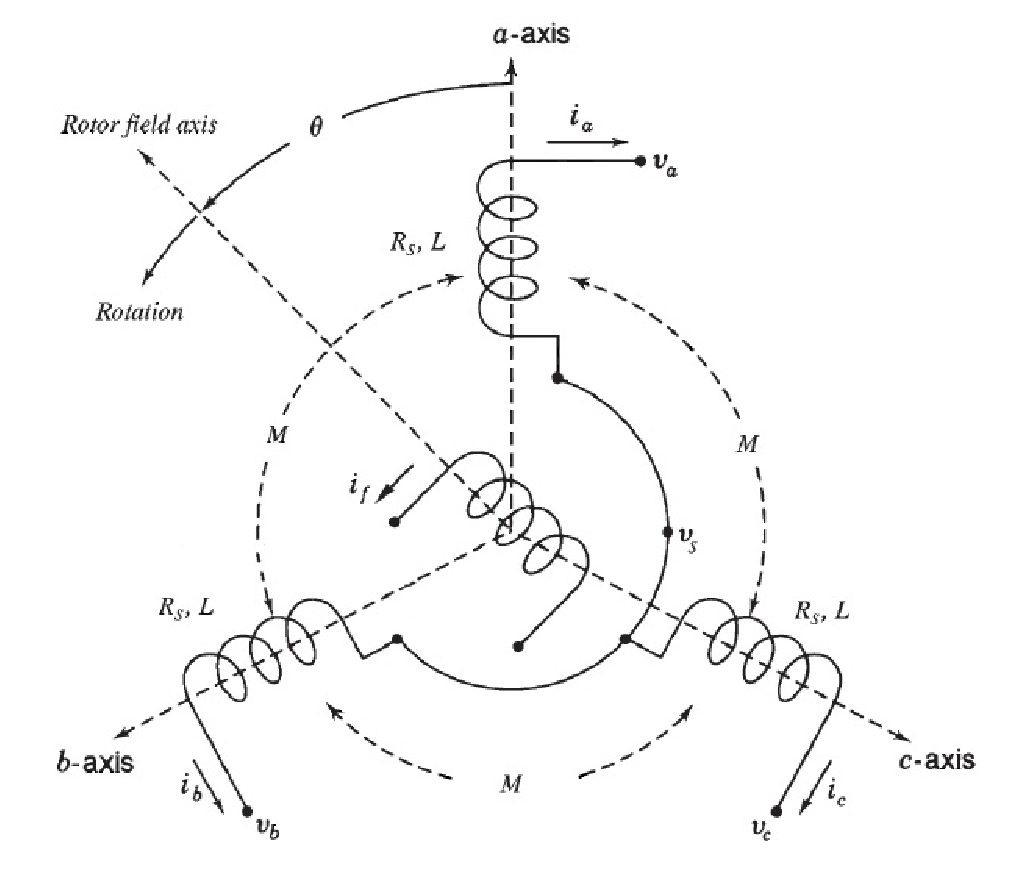
\includegraphics[scale=0.4]{SGStucture}
\par\end{centering}

\caption[Structure of an idealized three-phase round rotor synchronous generator]{Structure of an idealized three-phase round rotor synchronous generator,
modified from \cite{Grainger Stevenson2014} Figure 3.4}
\end{figure}


The mutual inductance between the rotor coil and each of the stator
coils varies with the rotor angle $\theta$ as follows:

\[
\left[\begin{array}{c}
M_{a,f}\\
M_{b,f}\\
M_{c,f}
\end{array}\right]=M_{f}\widetilde{\cos}\theta
\]


The flux linkage of the stator windings are

\[
\Phi=\left[\begin{array}{ccc}
L & -M & -M\\
-M & L & -M\\
-M & -M & L
\end{array}\right]i+M_{f}\widetilde{\cos}\theta
\]


Since there is no neutral, $i_{a}+i_{b}+i_{c}=0$, so the previous
equation can be rewritten as 

\[
\Phi=L_{s}i+M_{f}i_{f}\widetilde{\cos}\theta
\]


where $L_{s}=L+M$. We will assume that the rotor current is constant
(or equivalently, the rotor is composed of a permanent magnet). Each
stator terminal voltage is given by 

\begin{equation}
v=-R_{s}i-\frac{d\Phi}{dt}=-R_{s}i-L_{s}\frac{di}{dt}+e\label{eq:SGTerminalVlotage}
\end{equation}


where $e=\left[\begin{array}{c}
e_{a}\\
e_{b}\\
e_{c}
\end{array}\right]$ is the back electromotive force (EMF) due to the rotor movement given
by:

\begin{equation}
e=M_{f}i_{f}\dot{\theta}\widetilde{\sin}\theta\label{eq:emf}
\end{equation}


For synchronous generator with no load, the voltages at each terminal
will be sinusoidal functions. In order to convert the volteges (and
current) into a fixed value, we will apply Park's transformation:

\[
x_{dq0=}\left[\begin{array}{c}
x_{d}\\
x_{q}\\
x_{0}
\end{array}\right]=U(\theta)\left[\begin{array}{c}
x_{a}\\
x_{b}\\
x_{c}
\end{array}\right]=U(\theta)x_{abc}
\]


where $U(\theta)$ is the unitary matrix:

\[
U(\theta)=\sqrt{\frac{3}{2}}\left[\begin{array}{ccc}
\cos(\theta) & \cos(\theta-\frac{2\pi}{3}) & \cos(\theta-\frac{4\pi}{3})\\
\sin(\theta) & \sin(\theta-\frac{2\pi}{3}) & \sin(\theta-\frac{4\pi}{3})\\
\sqrt{\frac{1}{2}} & \sqrt{\frac{1}{2}} & \sqrt{\frac{1}{2}}
\end{array}\right]
\]


where $x_{abc}$ is some vector at abc coordinates, and $x_{dq0}$
is the same vector at the new coordinates.

Applying Park transformation to \eqref{eq:SGTerminalVlotage} leads
to

\begin{equation}
U(\theta)v-U(\theta)e=-R_{s}U(\theta)i-L_{s}U(\theta)\frac{di}{dt}\label{eq:SGTerminalVlotageAfetrPark}
\end{equation}


Using that 

\[
\frac{di_{dq0}}{d\theta}=U(\theta)\frac{di_{abc}}{d\theta}+\frac{dU(\theta)}{d\theta}i_{abc}=U(\theta)\frac{di_{abc}}{d\theta}+\left[\begin{array}{c}
i_{q}\\
-i_{d}\\
0
\end{array}\right]
\]


To calculate the time derivative of $i$:

\[
\dot{i}_{dq0}=\frac{di_{dq0}}{d\theta}\frac{d\theta}{dt}=U(\theta)\dot{i}_{abc}+\omega\left[\begin{array}{c}
i_{q}\\
-i_{d}\\
0
\end{array}\right]
\]


where $\omega=\dot{\theta}$.

We rewrite \eqref{eq:SGTerminalVlotageAfetrPark} as follows:

\begin{equation}
L_{s}\frac{d}{dt}\left[\begin{array}{c}
i_{d}\\
i_{q}\\
i_{0}
\end{array}\right]-L_{s}\omega\left[\begin{array}{c}
i_{q}\\
-i_{d}\\
0
\end{array}\right]=-R_{s}\left[\begin{array}{c}
i_{d}\\
i_{q}\\
i_{0}
\end{array}\right]+\left[\begin{array}{c}
e_{d}-v_{d}\\
e_{q}-v_{q}\\
e_{0}-v_{0}
\end{array}\right]\label{eq:idiqDynamics}
\end{equation}


Since there is no neutral connection, $i_{0}=0,$ hence $e_{0}=0$.
Applying Park transformation on \eqref{eq:emf} gives:

\[
\left[\begin{array}{c}
e_{d}\\
e_{q}
\end{array}\right]=-\sqrt{\frac{3}{2}}M_{f}\left[\begin{array}{c}
0\\
\omega i_{f}
\end{array}\right]
\]


We  denote $m=\sqrt{\frac{3}{2}}M_{f}$ 

Substitute this equation to \eqref{eq:idiqDynamics} gives:

\begin{equation}
\begin{array}{ccc}
L_{s}\frac{d}{dt}\left[\begin{array}{c}
i_{d}\\
i_{q}
\end{array}\right] & = & -R_{s}\left[\begin{array}{c}
i_{d}\\
i_{q}
\end{array}\right]+\omega L_{s}\left[\begin{array}{c}
i_{q}\\
-i_{d}
\end{array}\right]\\
 &  & -m\left[\begin{array}{c}
0\\
\omega i_{f}
\end{array}\right]-\left[\begin{array}{c}
v_{d}\\
v_{q}
\end{array}\right]
\end{array}\label{eq:idiqDynamicsWithExIf}
\end{equation}


The rotational dynamics of the rotor is given by the equation:

\begin{equation}
J\dot{\omega}=T_{m}-T_{e}-D_{p}\omega\label{eq:mechanicalPart}
\end{equation}


where $J$ is the moment of inertia of the rotor, $T_{m}$ is is the
mechanical torque which applies by the prime mover, $T_{e}$ is the
electromagnetic torque developed by the generator, and $D_{p}$ is
a damping factor, which consist of the viscous friction acting on
the rotor and the frequency droop from $\omega$ to the mechanical
torque of the prime mover, which added in order to control the frequency
of the generator.

$T_{e}$ can be found using energy consideration. The magnetic energy
stored in the generator is 
\[
\begin{array}{ccc}
E_{mag} & = & \frac{1}{2}\left(<i,\Phi>+i_{f}\Phi_{f}\right)\\
 & = & \frac{1}{2}\left(<i,L_{s}i>+Li_{f}^{2}\right)+M_{f}i_{f}<i,\widetilde{cos}\theta>
\end{array}
\]


The electromagnetic torque can be calculated as follows:

\[
T_{e}=\frac{\partial E_{mag}}{\partial\theta}|_{\Phi=const}=\frac{\partial E_{mag}}{\partial\theta}|_{i=const}
\]


\begin{equation}
T_{e}=M_{f}i_{f}<i,\frac{d\tilde{cos}\theta}{d\theta}>=M_{f}i_{f}<i,\tilde{sin}\theta>=-mi_{f}i_{q}\label{eq:electricTorque}
\end{equation}


Using  \eqref{eq:idiqDynamicsWithExIf}, \eqref{eq:mechanicalPart}
and \eqref{eq:electricTorque} we obtained:

\begin{equation}
\begin{array}{ccc}
\frac{d}{dt}\left[\begin{array}{c}
L_{s}i_{d}\\
L_{s}i_{q}\\
J\omega
\end{array}\right] & = & \left[\begin{array}{ccc}
-R_{s} & \omega L_{s} & 0\\
-\omega L_{s} & -R_{s} & -mi_{f}\\
0 & mi_{f} & -D_{p}
\end{array}\right]\left[\begin{array}{c}
i_{d}\\
i_{q}\\
\omega
\end{array}\right]\\
 &  & +\left[\begin{array}{c}
-v_{d}\\
-v_{q}\\
T_{m}
\end{array}\right]
\end{array}\label{eq:SGDynamics}
\end{equation}


This third order nonlinear dynamical system represents the dynamics
of a single synchronous generated with constant field current. 


\subsection{Model of a single generator connected to an infinite bus}

In this section we develop a model for single synchronous generator
which connected to an infinite bus. This section follows the work
describe in \cite{NatarajanWeiss2015}. The infinite bus is modeled
as tree phase AC voltage source. i.e the infinite bus is not affected
by the synchronous generator that connected to it. The reason for
this model is that the influence of a single synchronous generator
on a grid is very small. In general, the line that connect the synchronous
generator to the grid has its impedance that consist of resistance
and inductance, but since it is connected to the synchronous generator
in series, the $R_{s}$ and $L_{s}$ parameters can take into account
the impedance of both the synchronous generator and the line.

The infinite bus is modeled as voltage source. Thus, the voltage at
the synchronous generator terminals is

\begin{equation}
v=\left[\begin{array}{c}
v_{a}\\
v_{b}\\
v_{c}
\end{array}\right]=\sqrt{\frac{2}{3}}V\left[\begin{array}{c}
\cos(\theta_{g})\\
\cos(\theta_{g}-\frac{2\pi}{3})\\
\cos(\theta_{g}-\frac{4\pi}{3})
\end{array}\right]\label{eq:infBusVoltageABC}
\end{equation}


where $V$ is the grid voltage magnitude, and $\theta_{g}$ is the
grid phase. Lets define the angle $\delta$ which represent the difference
between the grid and the synchronous generator angles:

\[
\delta=\theta-\theta_{g}
\]


After applying Park transformation (which depends on $\theta$ which
is the synchronous generator phase) on \eqref{eq:infBusVoltageABC}
we have 

\begin{equation}
\begin{array}{ccc}
v_{dqo}=\left[\begin{array}{c}
v_{d}\\
v_{q}\\
v_{0}
\end{array}\right] & = & U(\theta)\sqrt{\frac{2}{3}}V\left[\begin{array}{c}
\cos(\theta_{g})\\
\cos(\theta_{g}-\frac{2\pi}{3})\\
\cos(\theta_{g}-\frac{4\pi}{3})
\end{array}\right]\\
 & = & -V\left[\begin{array}{c}
\sin(\delta)\\
\cos(\delta)\\
0
\end{array}\right]
\end{array}\label{eq:infBusVoltageDQO}
\end{equation}


It is easy to see that the dynamics of $\delta$ is 

\begin{equation}
\dot{\delta}=\omega-\omega_{g}\label{eq:deltaDynamics}
\end{equation}


where $\omega_{g}$ is the grid frequency. Substituting \eqref{eq:infBusVoltageDQO}
and \eqref{eq:deltaDynamics} into \eqref{eq:idiqDynamics} gives:

\begin{equation}
\begin{array}{ccc}
\frac{d}{dt}\left[\begin{array}{c}
L_{s}i_{d}\\
L_{s}i_{q}\\
J\omega\\
\delta
\end{array}\right] & = & \left[\begin{array}{cccc}
-R_{s} & \omega L_{s} & 0 & 0\\
-\omega L_{s} & -R_{s} & -mi_{f} & 0\\
0 & mi_{f} & -D_{p} & 0\\
0 & 0 & 1 & 0
\end{array}\right]\left[\begin{array}{c}
i_{d}\\
i_{q}\\
\omega\\
\delta
\end{array}\right]\\
 &  & +\left[\begin{array}{c}
V\sin(\delta)\\
V\cos(\delta)\\
T_{m}\\
\omega_{g}
\end{array}\right]
\end{array}\label{eq:SGDynamicsInfBus}
\end{equation}


This fourth order nonlinear dynamical system is the model for one
synchronous generator which connected to an infinite bus.


\section{Develop the improved swing equation for infinite bus:}

We separate the model in to a fast variable and a slow variable in
order to have singular perturbation analysis (see \cite{Khalil}).
The new dynamics form is:

\[
\left\{ \begin{array}{c}
\dot{x}=f(x,y,\epsilon)\\
\epsilon\dot{y}=g(x,y,\epsilon)
\end{array}\right.
\]


Where $x$ is the slow varying variable, $y$ is the fast varying
variable and $\epsilon$ is a small parameter.

In our case, assuming that $L_{s}$ is much smaller than the other
parameter, define $\epsilon$ as $L_{s}$, $x=\left[\begin{array}{c}
\omega\\
\delta
\end{array}\right]$, and $y=\left[\begin{array}{c}
i_{d}\\
i_{q}
\end{array}\right]$

and now 

\[
g(x,y,\epsilon)=\left[\begin{array}{cc}
-R_{s} & \omega L_{s}\\
-\omega L_{s} & -R_{s}
\end{array}\right]\left[\begin{array}{c}
\omega\\
\delta
\end{array}\right]+\left[\begin{array}{c}
V\sin(\delta)\\
V\cos(\delta)-mi_{f}\omega
\end{array}\right]
\]


We assume that $\epsilon$ is very small, meaning that $\epsilon\dot{y}=g(x,y,\epsilon)$
is much faster than $\dot{x}=f(x,y,\epsilon)$, and it will reach
it equilibrium (assuming that the equilibrium point exist and attractive)
almost instantly with regard to $x$.

The equilibrium point $y_{0}=\hat{y}(x,\epsilon=0)$ is the root of
$g(x,y,\epsilon)=0.$ 

The solution of this linear equation (in $\hat{y}$) is:

\[
\begin{array}{ccc}
\hat{y} & = & -\left[\begin{array}{cc}
-R_{s} & \omega L_{s}\\
-\omega L_{s} & -R_{s}
\end{array}\right]^{-1}\left[\begin{array}{c}
V\sin(\delta)\\
V\cos(\delta)-mi_{f}\omega
\end{array}\right]\\
 & = & \left[\begin{array}{c}
\frac{R_{s}V\sin(\delta)-L_{s}\omega\left(mi_{f}\omega-V\cos(\delta)\right)}{L_{s}^{2}\omega^{2}+R_{s}^{2}}\\
\frac{-R_{s}\left(mi_{f}\omega-V\cos(\delta)\right)-L_{s}V\omega\sin(\delta)}{L_{s}^{2}\omega^{2}+R_{s}^{2}}
\end{array}\right]
\end{array}
\]


Assuming that $R_{s}\ll L_{s}\omega_{g}$ and $R_{s}mi_{f}\ll L_{s}V$
, and assuming that our dynamics are close to the equilibrium, namely
$\omega\simeq\omega_{g}$. 

\begin{equation}
\hat{y}=\left[\begin{array}{c}
\hat{i}_{d}=\\
\hat{i}_{q}
\end{array}\right]=\left[\begin{array}{c}
\frac{V\cos(\delta)-mi_{f}\omega}{L_{s}\omega}=\\
-\frac{V\sin(\delta)}{L_{s}\omega}
\end{array}\right]\label{eq:ISEInfBusEstimatedCurrents}
\end{equation}


Now, substitute $\hat{y}$ in $\dot{x}=f(x,y,\epsilon)$ to have a
reduced model:

\[
\left\{ \begin{array}{c}
J\dot{\omega}\omega+D_{p}\omega\omega=-\frac{mi_{f}V\sin(\delta)}{L_{s}}+T_{m}\omega\\
\dot{\delta}=\omega-\omega_{g}
\end{array}\right.
\]


Wes assume that the income torque is due to fix mechanical power and
a correction factor for the viscose looses:

\[
T_{m}=\frac{P_{m}}{\omega}+D_{p}\omega_{g}
\]


and then the model is: 

\[
\left\{ \begin{array}{c}
J\dot{\omega}\omega+D_{p}\omega(\omega-\omega_{g})=P_{m}-\frac{mi_{f}V\sin(\delta)}{L_{s}}+\\
\dot{\delta}=\omega-\omega_{g}
\end{array}\right.
\]


This model is known as the \textit{improved swing equation} model,
see \cite{DePersiVanDerSchaft2016},\cite{ZhouOhsawa2009}.


\section{Simulations:}

In this section, we present a simulation that demonstrates that the
improved swing equation model is a good reduction for many cases,
but there are cases in which there is mismatch between the behavior
suggested by the improved swing equations model and the fourth order
model \eqref{eq:SGDynamicsInfBus}. For each simulation, we will show
the currents $i_{d}$ and $i_{q}$over time for both the fourth order
model and the improved swing equation model, where for the improved
swing equation model, we estimate these currents by \eqref{eq:ISEInfBusEstimatedCurrents}.
In addition we will show the frequency over time for the two models,
and the phase over time of the fourth order model and the improved
swing equation model.


\subsection{5KW SG}

\begin{figure}[h]
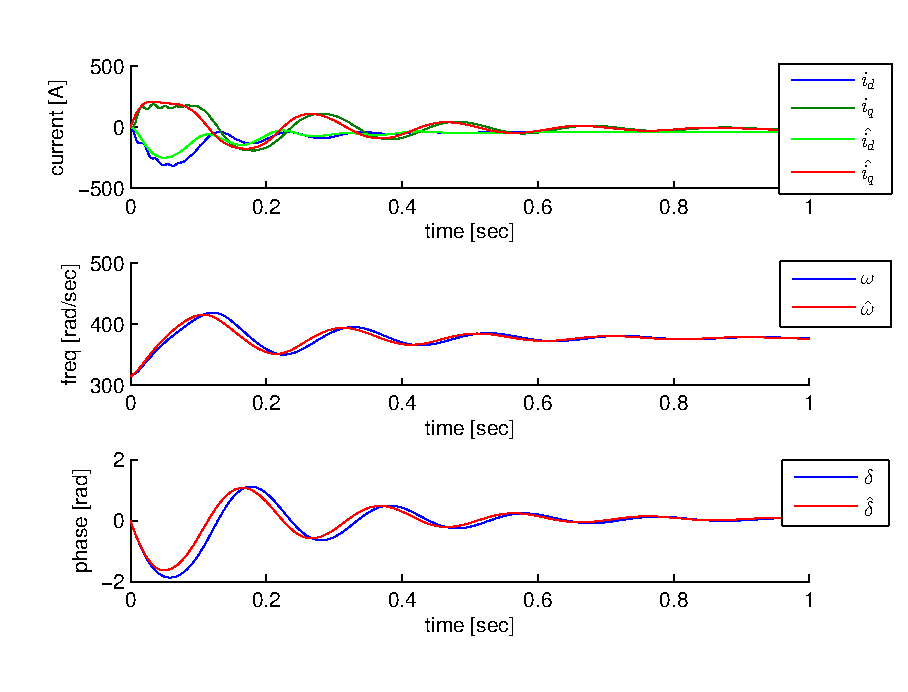
\includegraphics[scale=0.5]{sim5KWInfBus}

\caption{Simulation for infinite bus with single 5KW SG}
\label{fig:InfBusOne5KWSG}
\end{figure}


As shown in Figure \ref{fig:InfBusOne5KWSG}, simulations show that
for the 5KW SG, the behavior of the fourth order model and the reduced
model is almost the same. Although the currents at the reduced don't
have a ripple that the fourth order model has, both models converge
at the same rate with the same oscillations to the same equilibrium
point (The parameters for this simulation are $J=0.2$ {[}$kgm^{2}${]},
$D_{p}=1.7$ {[}$J/sec${]}, $R_{s}=0.152$ {[}$\Omega]$, $L_{s}=4.4$
{[}$mH${]}, $mi_{f}=1.05$ {[}$Vsec]$, $\omega_{g}=60\cdotp2\pi$
{[}$rad/sec${]}, $V=330$ {[}$V]$, $Pm=5$ {[}$kW${]}). 


\subsection{1MW SG}

\begin{figure}[h]
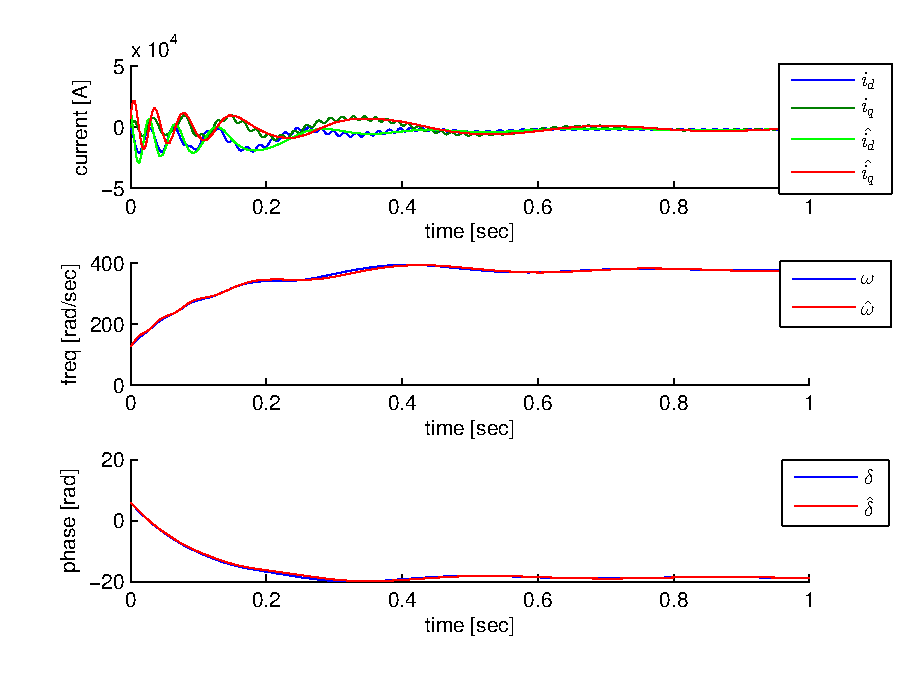
\includegraphics[scale=0.5]{sim1MWInfBus}

\caption{Simulation for infinite bus with single 1MW SG}
\label{fig:InfBusOne1MWSG}
\end{figure}


As shown in Figure \ref{fig:InfBusOne1MWSG}, simulations show that
for the 1MW SG, the behavior of the fourth order model and the reduced
model are still very similar. Although the fourth order model currents
are much rippled than the reduced model currents, both models converge
at the same rate with the same oscillations to the same equilibrium
point (The parameters for this simulation are $J=40.05$ {[}$kgm^{2}${]},
$D_{p}=337$ {[}$J/sec${]}, $R_{s}=0.4$ {[}$\Omega]$, $L_{s}=18$
{[}$mH${]}, $mi_{f}=1.79$ {[}$Vsec]$, $\omega_{g}=60\cdotp2\pi$
{[}$rad/sec${]}, $V=563$ {[}$V]$, $Pm=1$ {[}$MW${]}). 


\subsection{Non stable behavior of the reduced model}

\begin{figure}[h]
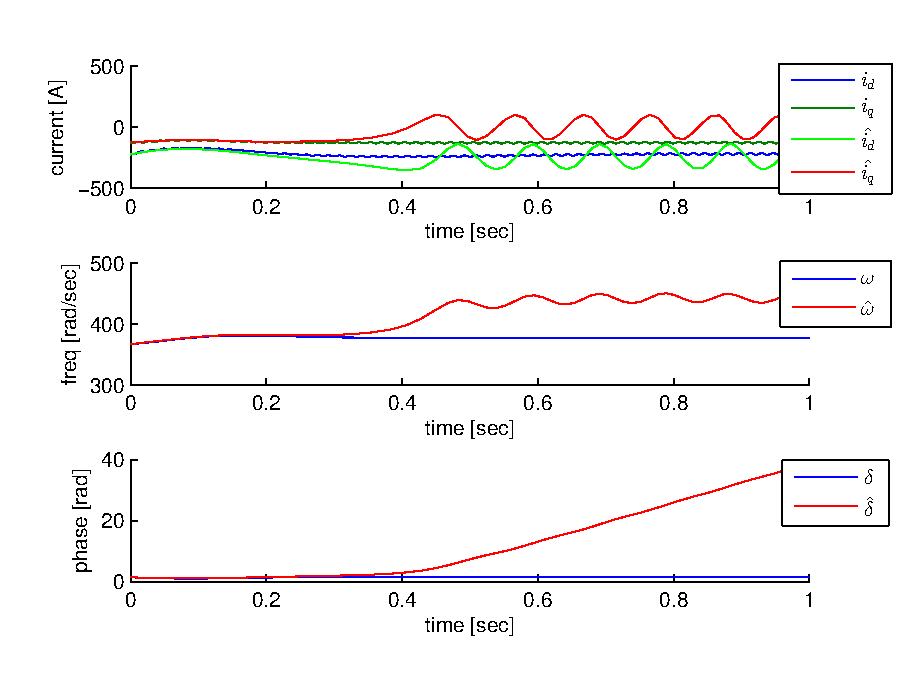
\includegraphics[scale=0.5]{simDiffBehavior1}

\caption{Simulation example that shows different behavior for the reduced model}
\label{fig:InfBusOne1DiffBehavior1}
\end{figure}


As shown in Figure \ref{fig:InfBusOne1DiffBehavior1}, simulations
show that for other parameters set (The parameters for this simulation
are $J=0.2$ {[}$kgm^{2}${]}, $D_{p}=1.7$ {[}$J/sec${]}, $R_{s}=0.152$
{[}$\Omega]$, $L_{s}=4.4$ {[}$mH${]}, $mi_{f}=1.05$ {[}$Vsec]$,
$\omega_{g}=60\cdotp2\pi$ {[}$rad/sec${]}, $V=200$ {[}$V]$, $Pm=50$
{[}$kW${]}) the behavior of the fourth order model and the reduced
model is significantly different. while the four order model is stable
(the eigenvalues of the Jacobian around the equilibrium point are:
\[
\left[-11.41+376.9i,-11.41-376.9i,-508+837i,-508-837i\right]
\]
 the reduced model is not stable (the eigenvalues of the Jacobian
around the equilibrium point are: $\left[-14.6+9.4979i,\:6.1-9.4i\right]$)
.


\subsection{Different region of attraction example}

\begin{figure}[h]
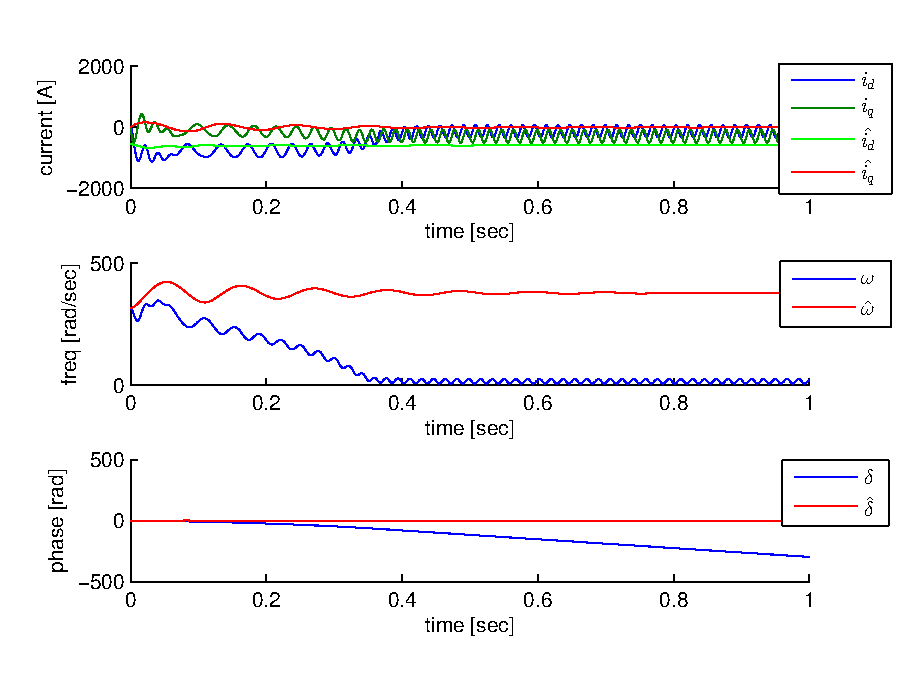
\includegraphics[scale=0.5]{simDiffRegionOFAttraction}

\caption{Simulation example that shows different behavior for the reduced model}
\label{fig:InfBusOne1DiffRegionOfAttraction}
\end{figure}


As shown in Figure \ref{fig:InfBusOne1DiffRegionOfAttraction}, simulations
show that for some parameters set (The parameters for this simulation
are $J=0.2$ {[}$kgm^{2}${]}, $D_{p}=1.7$ {[}$J/sec${]}, $R_{s}=0.152$
{[}$\Omega]$, $L_{s}=1.05$ {[}$mH${]}, $mi_{f}=3.5$ {[}$Vsec]$,
$\omega_{g}=60\cdotp2\pi$ {[}$rad/sec${]}, $V=330$ {[}$V]$, $Pm=5$
{[}$kW${]}) the initial condition of this simulation is within the
region of attraction of the reduced model, but outside the region
of attraction of the fourth model. That cause the fourth order model
to diverge while the reduce model converges to the equilibrium point. 


\section{Conclusions}

We have showed the relation between the fourth order model of SG connected
to an infinite bus and the improved swing equation model. Simulations
are carried out to show that the fourth order model gives rise to
a behavior that does not match what is suggested by the improved swing
equation. 


\section*{Acknowledgment}

The authors would like to thank...
\begin{thebibliography}{10}
\bibitem{SauerPai1998} P.~W.~Sauer and M.~A.~Pai, \emph{Power
Systems Dynamics and Stability}.\hskip 1em plus 0.5em minus 0.4em\relax
Stipes Publishing, Champaign, IL, 1997.

\bibitem{ZhongWeiss2011} Q.-C. Zhong and G. Weiss,\emph{ Synchronverters:
Inverters that mimic synchronous generator}.\hskip 1em plus 0.5em
minus 0.4em\relax IEEE Trans. Industr. Electronics, 58 (2011), pp.
1259-1267.

\bibitem{DePersiVanDerSchaft2016} P. Monshizadeh and C De Persis
and N. Monshizadeh and A. van der Schaft,\emph{ Nonlinear Analysis
of an Improved Swing Equation}.\hskip 1em plus 0.5em minus 0.4em\relax
Submitted in 2016.

\bibitem{DorflerBullo2012} F. Dorfler and F. Bullo,\emph{ Synchronization
and transient stability in power net- works and nonuniform Kuramoto
oscillators}.\hskip 1em plus 0.5em minus 0.4em\relax SIAM J. Control
and Optim., 50 (2012), pp. 1616-1642.

\bibitem{PorcoDorfleBullo2013}J. W. Simpson-Porco and F. D�rfler
and F. Bullo, \emph{Synchronization and power sharing for droop-controlled
inverters in islanded microgrids}.\hskip 1em plus 0.5em minus 0.4em\relax
Automatica, 49(2013), pp. 2603\textendash 2611.

\bibitem{Khalil}H.K. Khalil, \emph{Nonlinear Systems} (third edition).\hskip
1em plus 0.5em minus 0.4em\relax Prentice Hall, New Jersey, 2002.

\bibitem{Kundur}P. Kundur, \emph{Power System Stability and Control}.\hskip
1em plus 0.5em minus 0.4em\relax McGraw-Hill, New York, 1994.

\bibitem{CaliskanTabuada2014}S.Y. Caliskan and P. Tabuada, \emph{Compositional
transient stability analysis of multimachine power networks},\hskip
1em plus 0.5em minus 0.4em\relax IEEE Trans. Control of Network Systems,
1 (2014), pp. 4-14.

\bibitem{Grainger Stevenson2014}J.J. Grainger and W.D. Stevenson,
\emph{Power Systems Analysis},\hskip 1em plus 0.5em minus 0.4em\relax
McGraw-Hill, New York, 1994.

\bibitem{NatarajanWeiss2015}V. Natarajan and G. Weiss, \emph{Almost
global asymptotic stability of a grid- connected synchronous generator},\hskip
1em plus 0.5em minus 0.4em\relax submitted in 2015.

\bibitem{ZhouOhsawa2009}J. Zhou and Y. Ohsawa, \emph{Improved swing
equation and its properties in synchronous generators}, \hskip 1em
plus 0.5em minus 0.4em\relax Circuits and Systems I: Regular Papers,
IEEE Transactions ,56(1), pp. 200\textendash 209, 2009.\end{thebibliography}

\end{document}
